\chapter{Time-memory-data tradeoff using Hellman tables}
\label{chapter:tmdto-hellman}

\indent \textbf{\textit{Summary.}} In sections \ref{sec:bg-keystream-attack} and \ref{sec:bg-tags-attack}, we described two TMTO attacks designed particularly for stream ciphers. They take into account two set of states: one set computed during the precomputation phase, and the other set containing states traversed during the attack phase. A common state is desired to occur between these two sets, and the parameters of the attack are chosen in order to have high chances of this occurrence.

The attacks we describe in this and the next chapter are different from these two attacks. These attacks were originally designed for block ciphers. By making certain changes to the attack schemes, tradeoff attacks for stream ciphers are proposed. The Hellman attack is the one we consider in this chapter. First, the original attack for block ciphers is described. Then using this, Biryukov and Shamir attack is described for stream ciphers with their tradeoff equation. Further, we propose a general tradeoff equation for the attack and present attack results for parameters selected according to this general tradeoff equation.

\section{Hellman tables for block ciphers}

A block cipher is an encryption algorithm, which takes in a plaintext block of $n$ bits (called the block size) and a key of $k$ bits, and returns a ciphertext block of $n$ bits. Figure \ref{fig:block-cipher} illustrates a simple block cipher, with plaintext, ciphertext and key represented by $P$, $C$ and $K$ respectively. The encryption function is denoted by $E$ such that $C$ = $E_K(P)$ and implying encryption of $P$ under $K$.

\begin{figure}[ht!]
	\centering
		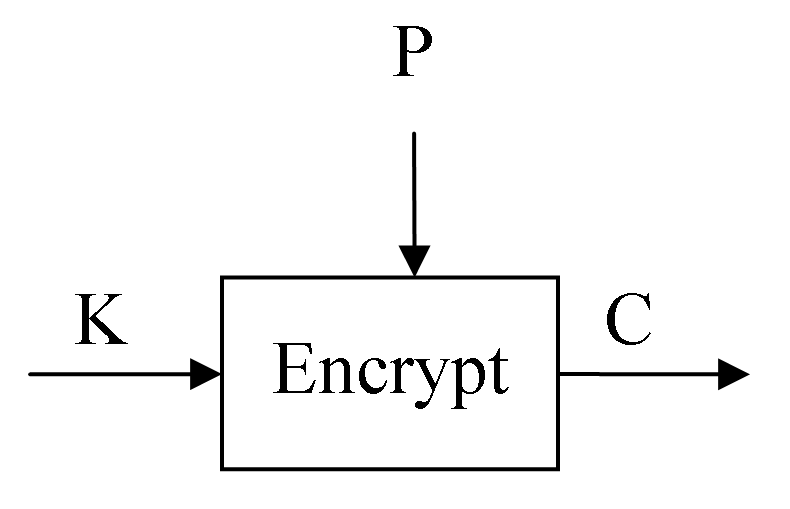
\includegraphics[width=2in]{./figures/block-cipher.PNG}
	\caption{A block cipher}	
	\label{fig:block-cipher}
\end{figure}

We first present the idea of the attack under certain ideal assumptions. Later we build upon this idea by considering the practical problems and their mitigation through a more practical attack.

\subsection{The ideal TMTO attack}
In the general scenario of an attack on block ciphers, the attacker has knowledge of a particular plaintext block $P$ and the corresponding ciphertext block $C$. The goal is to find $K$, using which the attacker can decrypt the ciphertext corresponding to unknown plaintext. For simplicity we assume the size of $K$ to be equal to the block size of $n$ bits. Then consider the following precomputation phase.\\

\noindent \textit{\textbf{Precomputation phase.}} An $n$ bit value is randomly selected and denoted by $SP$ for a starting point. Using $SP$ as a key (denoted by $K_0$), encryption of $P$ is performed. The ciphertext obtained from this encryption is then used as the key (denoted by $K_1$) for the subsequent round of encryption of $P$. This procedure is iterated over a total number of $t$ encryptions, yielding the key $K_t$ at the end. The key $K_t$ is called an end point, and is denoted by $EP$. Moreover, the sequence of encryptions starting from $SP$ to $EP$ is called a \emph{chain} and is illustrated in the figure \ref{fig:block-cipher-single-chain}. Equations for the $t$ encryptions are also shown below. 

\begin{align*}
& & K_0 &= SP & & & &\\
1&. & K_1 &= E_{K_0}(P) & & & &\\
2&. & K_2 &= E_{K_1}(P) & & & &\\
& & &\vdots & & & &\\
(t-1)&. &K_{t-1} &= E_{K_{t-2}}(P) & & & &\\
(t)&. &K_{t} &= E_{K_{t-1}}(P) & & & &\\
& & EP &= K_{t} & & & &\\
\end{align*}

\begin{figure}[ht!]
	\centering
		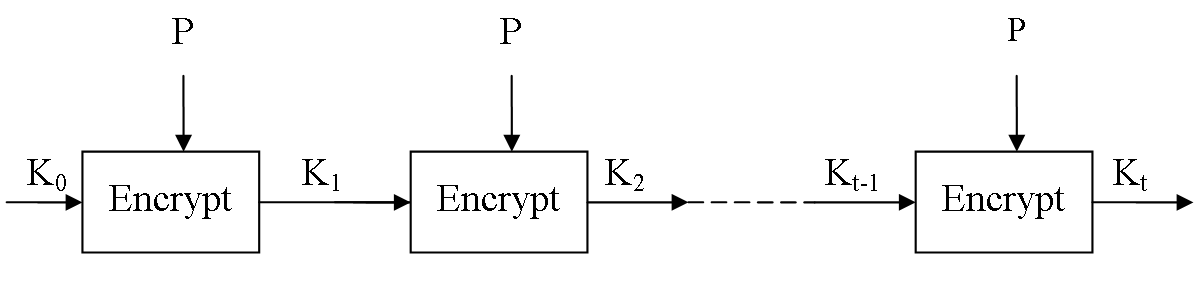
\includegraphics[width=5.5in]{./figures/block-cipher-single-chain.PNG}
	\caption{A chain of encryptions}	
	\label{fig:block-cipher-single-chain}
\end{figure}

During the precomputation phase, the goal is to cover the entire key space such that all possible keys are used atleast once to encrypt $P$. A single chain covers a total of $t$ distinct keys. Though the chain contains a total of $(t+1)$ keys starting from $K_0$ to $K_{t}$, only the first $t$ keys are useful during the attack phase. This we shall explain later, and for the moment we note that only $t$ keys are represented in the chain.

An appropriate length $t$ of the chain is chosen so that no key repeats in the chain. Repetition is not desired since once a key reappears, subsequent keys would also repeat, adding no extra information to the chain. Hence, the size of the chain is restricted, and more than one chains are created instead. 

Lets say $m$ more such chains are needed to cover all possible keys. If we consider the ideal case in which each chain contains $t$ distinct keys, then we have $m$ = $2^n/t$. For each chain, we select a random starting point $SP_j$ and compute the end point $EP_j$, for $1 \leq j \leq m$, as shown in figure \ref{fig:single-chain}. Only the pairs $(SP_j,EP_j)$ are then stored in a hashtable, with $EP_j$ as the hashkey and $SP_j$ as the corresponding hashvalue. All the chains representing such a table structure are illustrated in the figure \ref{fig:naive-hellman-table}. We call this arrangement as the ideal case precomputation table structure. 

\begin{figure}[ht!]
	\centering
		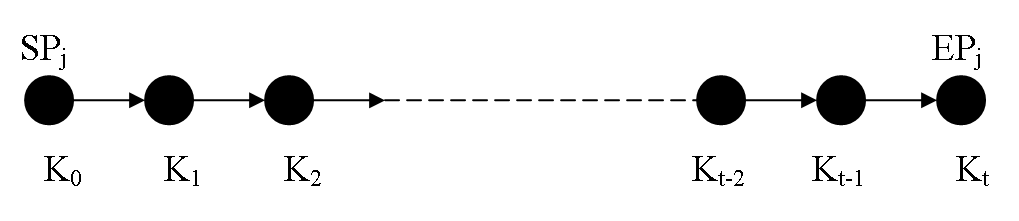
\includegraphics[width=4in]{./figures/single-chain.PNG}
	\caption{A single chain of encryptions represented by the pair $SP_j$ and $EP_j$}	
	\label{fig:single-chain}
\end{figure}

\begin{figure}[ht!]
	\centering
		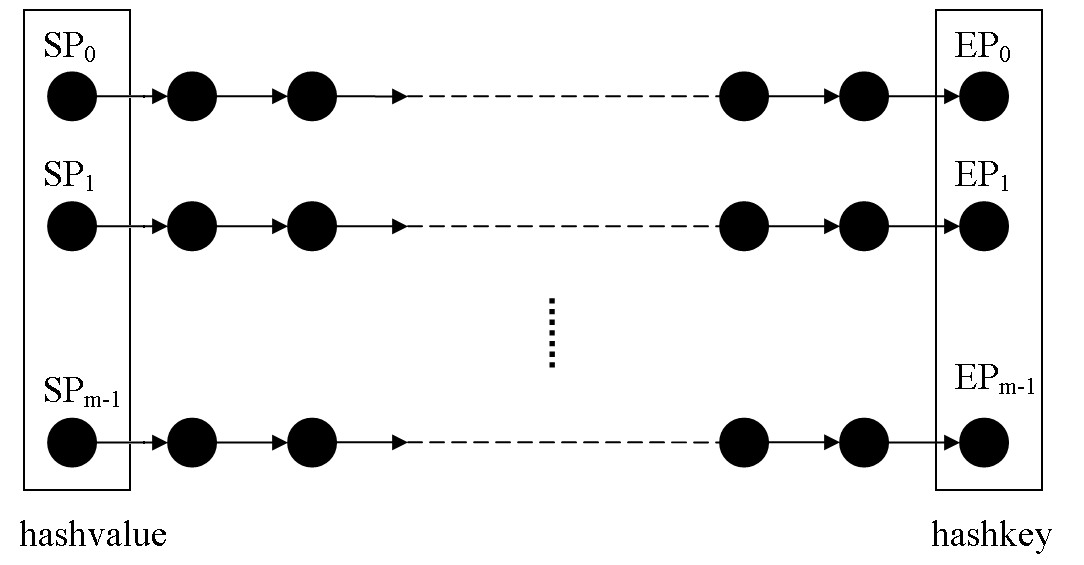
\includegraphics[width=4.5in]{./figures/naive-hellman-table.PNG}
	\caption{An ideal case precomputation table structure}	
	\label{fig:naive-hellman-table}
\end{figure}

We now compute $M$ and $P$ for the precomputation phase. The size of the memory required for storing all the chains would be of the order of $m$ as for each of the $m$ chains, a constant number of elements ($SP$ and $EP$) are stored. Thus we have $M$ = $m$. Also, as there are $mt$ encryptions performed in the entire table, the precomputation time is given by $P$ = $mt$. The assumption in the ideal case then is that precomputation covers all the possible $2^n$ keys, hence $P$ = $2^n$.\\

\noindent \textit{\textbf{Attack phase.}} It is easy to see that if the required key $K$ exists among the first $t$ keys in any chain, the ciphertext $C$ would also exist in the chain. The possible locations of $K$ thus in every chain are from $K_{j,0}$ to $K_{j,t-1}$. The key $K_{j,t}$ is not considered to be a possible key since it is not used in the encryption of $P$. Or in other words, the ciphertext obtained from $K_{j,t}$ is not computed and stored in the chain, hence it cannot be matched with the available ciphertext $C$. So, there are $t$ possible values for $K$ in every chain. Looking at this from the perspective of $C$, there are also $t$ possible ciphertexts in every chain that can match $C$. These $t$ ciphertexts correspond to each of the $t$ keys and range from $K_{j,1}$ to $K_{j,t}$.

The first possibility is that $C$ lies in $t^{th}$ column of any one of the $m$ chains. This is true only if $C$ equals some $EP_j$ stored in the hashtable. In such a case $K_{j,t-1}$ is the key we are looking for. To find this key, we retrieve $SP_j$ corresponding to $EP_j$ from the hashtable and perform $(t-1)$ encryptions on $P$, using $SP_j$ as the key for first encryption followed by the ciphertext from one encryption as key for next encryption. After $(t-1)$ encryptions the desired key $K_{j,t-1}$ is obtained. 

If $C$ does not match any of the $EP_j$, the next possibility is that $C$ lies in the $(t-1)^{th}$ column of some chain. If this is indeed the case, then $X$ = $E_{C}(P)$ must match with some $EP_j$. On a match, we know that the key $K_{j,t-2}$ is the required key. To find out $K_{j,t-2}$, we retrieve $SP_j$ corresponding to the matched $EP_j$ and perform $(t-2)$ encryptions. 

If none of the $EP_j$ matches with the evaluated $X$, we explore the possibility of $C$ lying in the remaining columns, one by one.

If $C$ exists in any chain, then the time taken to find $K$ is the same as the length of each chain. Assuming $C$ exists in the $r^{th}$ column such that  $2 \leq r \leq t$, then $X$ is computed by performing $(t-r)$ encryptions in the following way.

\begin{align*}
& & K_r &= C & & & &\\
1&. &K_{r+1} &= E_{K_r}(P)  & & & &\\
2&. &K_{r+2} &= E_{K_{r+1}}(P) & & & &\\
& & &\vdots & & & &\\
(t-r) &. &K_{r + (t-r)} &= E_{K_{r + (t-r-1)}}(P) & & & &\\
& & X &= K_{r + (t - r)} = K_t & & & &\\
\end{align*}

If $X$ matches an $EP_j$, then $(r-1)$ encryptions are performed to retrieve the key $K_{r-1}$. So in all, the number of encryptions performed is $(t-r) + (r-1)$ = $(t-1)$. Thus, the attack time is of the order of $t$ and our attack parameter $T$ = $t$.\\

\noindent \textit{\textbf{Problems with above approach.}} The approach described above is an ideal case, and some serious problems exist with it.

\begin{enumerate}

\item We have assumed that the length of $K$ is equal to the block size. This assumption does not hold for practical block ciphers, and thus we need to design a solution considering different key length and block size. Generally, the block size is larger than the key length. Thus a reduction function $R$ is required for the conversion of $n$ bits of $C$ to $k$ bits of $K$, where $n > k$. 

% some example reduction functions

During precomputation, the encryption function is replaced with the new function, which performs encryption and reduction to give the new key. This function is called the \emph{mapping function} (denoted by $f$), since it maps one key to another in the same keyspace. Such a mapping function is shown in figure \ref{fig:mapping-function}. 

\begin{figure}[ht!]
	\centering
		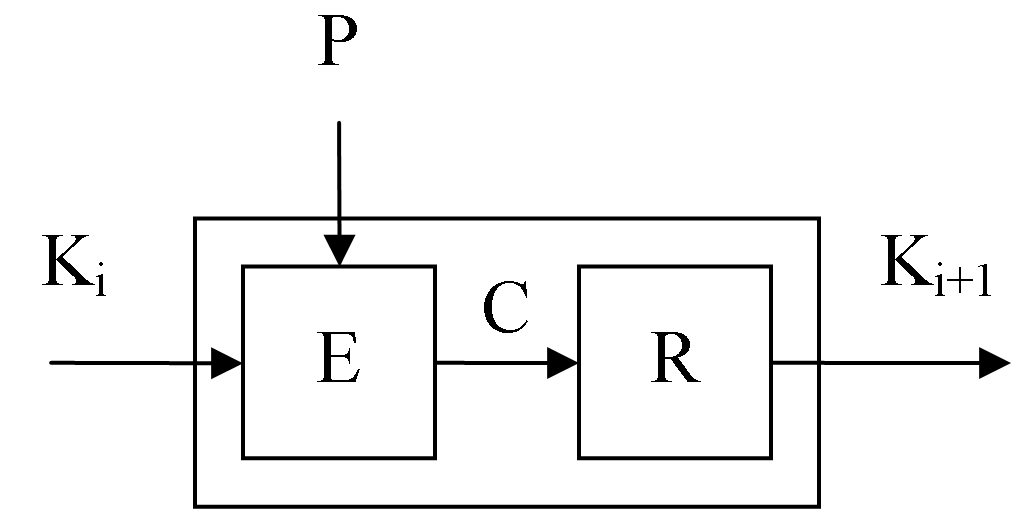
\includegraphics[width=3in]{./figures/mapping-function.PNG}
	\caption{Mapping function for block ciphers}	
	\label{fig:mapping-function}
\end{figure}

The function can also be represented in notation as follows, where $R$ stands for the reduction function.

\begin{center}
$K_{i+1}$ = $f(K_i)$ = $R(E_{K_i}(P))$\\
\end{center}

\item A much more serious problem in the ideal case is the assumption that all possible keys exist in the table structure and that no key is repeated. It is desired that all keys are covered, but practically this is hard to achieve. As more and more keys exist in the table, repetition of keys becomes frequent. The rate of repetitions grows exponentially after a certain number of keys making inclusion of new keys difficult in the table. This claim is can be proved using equation \ref{eq:bday-paradox2} of the birthday paradox.

Suppose we have $m$ chains with $t$ keys each so far in the table. A new chain is then added to the table. The total number of keys existing in the table are $mt$ while $t$ more keys are added through the new chain. We are interested in restricting $m$ and $t$ so that there is no common key between the $m$ chains and the new chain. According to the variant of the birthday paradox, the product of the sizes of these two sets should be less than or equal to the keyspace size, in order to have a high probability that no common key exists. Then, we have 

\begin{center}
$mt \times t \leq 2^n$\\
$mt^2 \leq 2^n$\\
\end{center}

If the $<$ condition is removed, then we have an upper bound on the value of $mt^2$ called the \emph{table stopping rule} and represented by the condition 
$mt^2 = 2^n$. 

In the ideal case described above, number of keys covered in the $m$ chains is $2^n$, which implies $mt = 2^n$. If we use this equation in estimating the value of $mt^2$, it can be seen that $mt^2$ is much greater than $2^n$. This is not allowed according to the table stopping rule, and thus lots of keys would repeat in our ideal table structure. Repetition of keys gives rise to the problems of \emph{collision and merge} during the precomputation phase and \emph{false alarms} during the attack phase. We explain these two problems below.
\end{enumerate}

\noindent \textit{\textbf{Collision and merge.}} Consider any two chains in the ideal precomputation table structure. If there is a common key $K_c$ existing in both the chains, then the sequence of keys appearing after $K_c$ would be the same in both chains, as shown in figure \ref{fig:collision-merge}. There would be overlapping keys in the two chains resulting in wastage of precomputation time since they add no extra information to the chains. Such a situation is called collision which consequently results in a merge.\\

\begin{figure}[ht!]
	\centering
		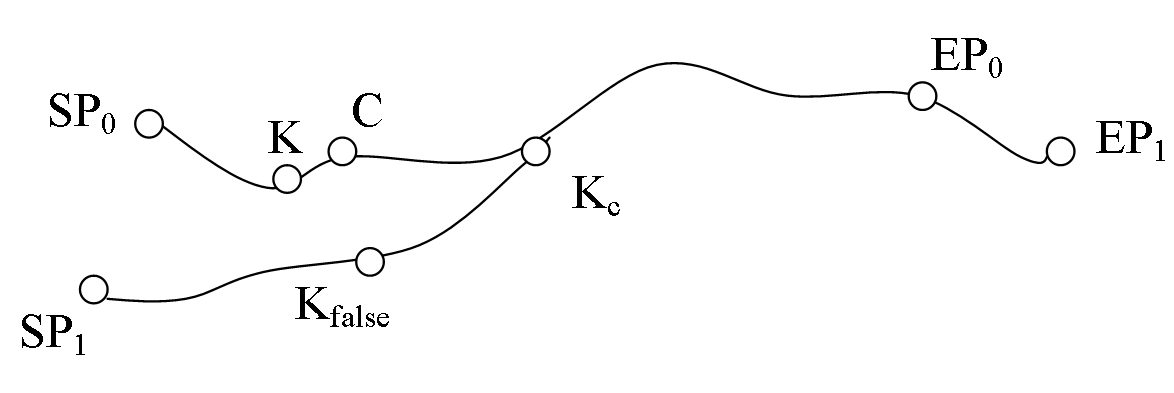
\includegraphics[width=4.5in]{./figures/collision-merge.PNG}
	\caption{Two chains which collide and consequently merge}	
	\label{fig:collision-merge}
\end{figure}

\noindent \textit{\textbf{False alarms.}} Colliding and merging chains during precomputation affect the attack phase as well. Consider the same example of the two chains colliding at $K_c$. Suppose that the required key $K$ appears in the first chain as shown in figure \ref{fig:collision-merge}. During the attack phase keys are computed starting from $C$ till one of the key matches an end point in the hashtable. 
In the example, a match would occur at $EP_1$ since $EP_1$ is one of the keys in the path from $C$ to $EP_0$ and $EP_1$ exists in the hashtable. The hashtable returns the starting point $SP_1$ for the match, and thus a key is derived from $SP_1$ ($K_{false}$). This key is different from the desired key $K$ since it lies in a different chain. This situation occurs as the two chains collide and merge and it said to be a \textit{false alarm}.

The occurrence of false alarms can be easily checked and ignored. It is expected that the ciphertext obtained by encrypting $P$ under the derived key be the same as $C$. The ciphertext obtained using $K_{false}$ is not the same as $C$ as both the keys are different. This confirms that $K_{false}$ is not the right key. The only problem with false alarms is that they waste time during the attack phase and thus increase the attack time for finding the correct key.\\

\noindent \textit{\textbf{Solving the problem of collision.}} The inclusion of reduction function does not help in solving the problem of collision. Collisions still have the same effect if mapping function $f$ is used instead of encryption function $E$. But, if we use different reduction functions (hence, different mapping functions) for two colliding chains, the two chains do not merge and produce different keys from the colliding point $K_c$. Even though the ciphertext computed from the colliding key would be same, different reduction functions in the two chains ensure different keys, thus preventing merging of the chains. Such a scenario is shown in figure \ref{fig:collision-not-merge}. 

\begin{figure}[ht!]
	\centering
		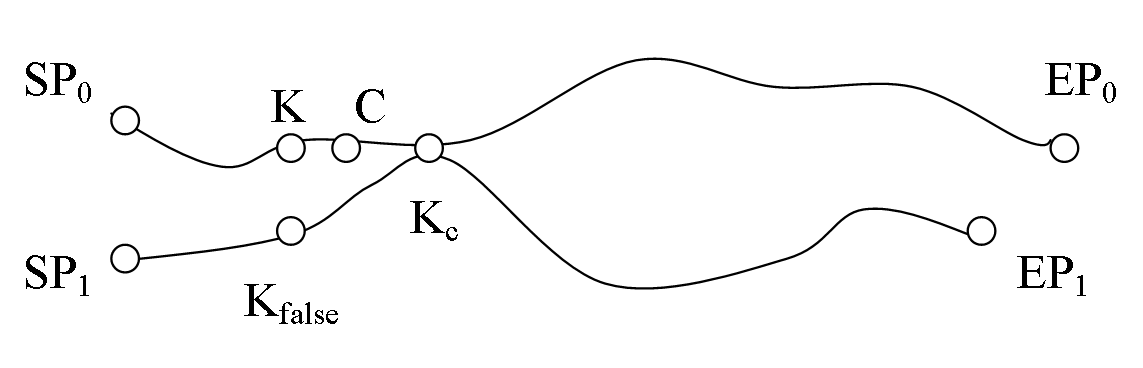
\includegraphics[width=4.5in]{./figures/collision-not-merge.PNG}
	\caption{Two chains which collide but do not merge}	
	\label{fig:collision-not-merge}
\end{figure}

As shown, the two chains terminate at different end points. As a result, when a match occurs during the attack phase, the correct starting point is retrieved from the hashtable and consequently the correct key is obtained. 

But practically, using $m$ different mapping functions for building the table has problems. Stamp and Low quote in \cite{stamp2007acb} that having $m$ mapping functions makes storage of these functions resource intensive, and thus that it's not a good idea. An apparent and more serious problem though, with having $m$ mapping functions, is that the attack phase would run for a long time. During the attack phase, the given $C$ must be evaluated for all the different mapping functions because the attacker does not know the chain in which $C$ appears. The attack time in such a case becomes proportional to $mt$. 

In any case, the idea of having different mapping functions for each chain is not feasible. But, the use of different mapping function provides a basis for a more practical table structure for block ciphers. 

\subsection{The practical TMTO attack}

Based on various ideas gathered from the previous section, the idea of Hellman tables \cite{hellman1980ctm} is presented here. The two important features of Hellman tables are the following,

\begin{enumerate}
\item There are multiple tables in the precomputation, as compared to the previously considered one big table. The total number of tables is denoted by $r$. Each table has a different mapping function, and thus collision occurring among chains belonging to different tables do not result in a merge.

\item In order to reduce the possibility of collisions occurring among chains within same tables, the size of each table is restricted in accordance with the \emph{table stopping rule}. Hence the relation $mt^2$ = $2^k$ must hold\footnote{We use $k$ here instead of $n$ since $n$ and $k$ are considered different, which is why the mapping function is used in the first place}.
\end{enumerate}

We describe in detail the precomputation and attack phase for the TMTO attack using the Hellman tables.\\
% need some thing more here.

\noindent \textit{\textbf{Precomputation phase.}} First, $r$ different random reduction functions are chosen, say \mbox{$R_1$, $R_2$, \ldots , $R_r$}. Using each of these functions, $r$ tables are created in the same way as described for the ideal case. Each of the $r$ tables consist of $m$ chains with $t$ keys and use mapping function $f_i$. Also, for each table, a different hashtable is created such that the starting and end points of the chains from that table are stored in the corresponding hashtable. Such a table structure is shown in figure \ref{fig:hellman-tables}, which is taken from \cite{oechslin:mfc}.

An important observation can be made from the figure: the number of computations in a chain is $(t-1)$, and not $t$ as we have been discussing. The same scene is observed in the discussion of Hellman tables in \cite{stamp2007acb} as well. With $(t-1)$ computations, $(t-1)$ keys exist in each chain. If $t$ is large as compared to 1, then $(t-1) \approx t$. Hence in these references, the number of keys in every chain is assumed to be $t$ for all analysis. On the other hand, we have assumed exactly $t$ keys per chain for the analysis and have also implemented the same.

\begin{figure}[ht!]
	\centering
		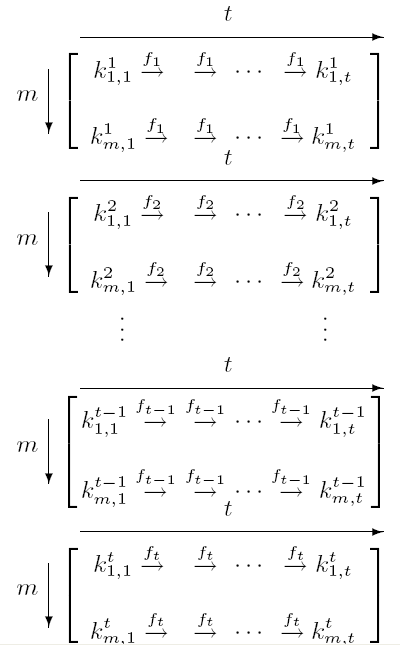
\includegraphics[width=3in]{./figures/hellman-tables.PNG}
	\caption{Structure of Hellman tables \cite{oechslin:mfc}}	
	\label{fig:hellman-tables}
\end{figure}

The equations for creating the keys in the chain $j$ of table $i$ are shown below. The mapping function is denoted by $f_i$ and the reduction function by $R_i$.
\begin{align*}
& & K_{j,0} & = SP_j & & & &\\
1&. &K_{j,1} & = R_i(E_{K_{j,0}}(P)) & & & &\\
2&. &K_{j,2} & = R_i(E_{K_{j,1}}(P)) & & & &\\
& & &\vdots & & & &\\
(t-1)&. &K_{j,t-1} & = R_i(E_{K_{j,t-2}}(P)) & & & &\\
(t)&. &K_{j,t} & = R_i(E_{K_{j,t-1}}(P)) & & & &\\
& & EP_j & = K_{j,t} & & & &
\end{align*}

The time for precomputation is proportional to the number of computations that are done in all the tables, which is $mtr$. Hence, $P$ = $mtr$. Also, corresponding to each table, $m$ $(SP, EP)$ pairs exist in the hashtable. Hence, total number of pairs in the hashtables is $mr$, resulting in required precomputation memory of order $M$ = $mr$.\\

\noindent \textit{\textbf{Attack phase.}} During the attack phase, ciphertext $C$ is searched through each of the $r$ tables one by one. Let's consider the case in which $C$ is searched through a particular table $i$. 

First, $X$ is computed using the reduction function as, $X$ = $R_i(C)$. $X$ is then matched with the end points of the table. If $X$ matches with the end point $EP_{j}$ of the $j^{th}$ chain, it means that the desired key lies in the $(t-1)^{th}$ column of that chain. $SP_{j}$ is retrieved from the hashtable (for table $i$) and $(t-1)$ computations are performed using $f_i$ to obtain the key in the $(t-1)^{th}$ column. We call this key $K_p$, $p$ standing for the possible key. If the ciphertext derived using $K_p$ is the same as $C$, then $K_p$ is the key we are looking for. Otherwise, we know that it is a case of false alarm. 

On the other hand, if $X$ does not match with any end point, $X$ is replaced with $f_i(X)$ and again matched with the end points. If there is a match, then the possible key appears in the $(t-2)^{th}$ column. Just as before, $SP_{j}$ is retrieved from the hashtable and $(t-2)$ computations of $f_i$ are performed to obtain $K_p$. Occurrence of false alarm is checked in the same way, confirming if $K_p$ is the desired key or not. 

$X$ is iteratively replaced by $f_i(X)$ for a maximum $(t-1)$ times, after which the same search procedure is performed on the next table. If there is a match, and if it is not a false alarm, then the correct key is obtained and the attack is terminated. 

In the worst case, $K$ is found after searching through all the tables. Searching a single table requires $t$ computations in the worst case. Hence, the attack time is proportional to $rt$. This implies that the order of the attack time is $T$ = $rt$.\\

\noindent \textit{\textbf{Tradeoff equation.}} We have derived the following relations for $M$ and $T$ so far, 
\begin{center}
$M = mr$\\
$T = rt$\\
\end{center}
Then, we have the table stopping rule,
\begin{center}
$mt^2 = 2^k$\\
\end{center}
Further, it is required that all the possible keys are covered in the Hellman tables. Since the number of keys computed during the precomputation is $mtr$, we require
\begin{align*}
mtr = 2^k
\end{align*}
From the last two equations, we have $r$ = $t$. Hence, the number of tables is equal to the length of each chain. Eliminating $m$ and $t$ from the relations for $M$ and $T$, we get the following tradeoff equation,
\begin{align}
\label{eq:hellman-block} M^{2}T = 2^k
\end{align}
The parameter $P$ now becomes $mt^2$ after replacing $r$ with $t$.\\ 

\noindent \textit{\textbf{Analysis.}} So how are Hellman tables better than a brute-force or precomputed ciphertext attack? Table \ref{tab:hellman-tmto-comparison} shows the order of precomputation time, precomputation memory and attack time for these three schemes. 

In the table, $c$ indicates a constant. The tradeoff attack reduces precomputation memory from $2^k$ in case of precomputed ciphertext attack to $M$. When compared with the brute-force attack, tradeoff attack reduces attack time from $2^k$ to $T$. Since both $M$ and $T$ are less than $2^k$ (from equation \ref{eq:hellman-block}), the tradeoff attack improves precomputation memory and attack time requirements. The only disadvantage of this attack, as also shown in the \mbox{table}, is in terms of the precomputation time. The tradeoff attack still requires precomputation time of the order of $2^k$.

\begin{table}[ht!]
\begin{center}
\begin{tabular}{c|c|c|c}
													&		Pre. time		& Pre. memory	& Attack time		 \\ \hline
Brute-force 							&		$-$		& $c$	 	& $2^k$		\\ \hline
Precomputed ciphertext		&		$2^k$	& $2^k$	& $c$		 	\\ \hline
TMTO using Hellman tables	&		$2^k$	& $M$ & $T$ 			\\
\end{tabular}
\end{center}
\caption{Performance of TMTO attack with Hellman tables}
\label{tab:hellman-tmto-comparison}
\end{table}

\section{Hellman tables for stream ciphers}

Hellman tables for block ciphers have been used for mounting tradeoff attacks on stream ciphers by Biryukov and Shamir in \cite{biryukov2000ctm}. Stream ciphers have a different working principle, and thus certain modifications in the original Hellman tables are proposed for them. 

Using Hellman tables an attacker can find the secret key $K$ if and only if the known plaintext $P$ is used in constructing the tables. Hence in a way, the tables are \emph{static} and cannot be re-used if a different plaintext and ciphertext pair for the same key are known. The tables can only be re-used if the same plaintext $P$ is later encrypted using a different key; say, during a different run of the protocol using the block cipher.

In addition, one of the important goals while constructing the tables for block ciphers is to cover all the possible keys. This is so, because a key can be found only when it is available in one of the tables. If the key does not exist, it can never be found as the ciphertext obtained using the key would not match in the tables. If the ciphertext matches, it would only turn out to be a different key which gives the same ciphertext as the correct key. 

Tables for stream ciphers differ from those for block ciphers based on these grounds. Precomputation done for stream ciphers (as we have already seen in chapter \ref{chap:bgtmto}) are not bound to a particular plaintext. The precomputation is general in nature containing mappings from prefix to state and can be re-used any number of times for keystream from different keys. Once a match is found, the current state of the LFSR is determined and it is then reversed to obtain the initial state. After this, the specific initialization parameters are used in finding the key from the initial state.

Also, stream ciphers move through a number of internal states while generating the output keystream. If the attacker is able to find any one of these internal states, the initial state is recovered and thus the key. The attacker has knowledge of \emph{data}, which comprises of subsequences of the keystream or the prefix of each of the internal state that occurs while generating the keystream. Using this data, several attempts of matching the current state in the precomputed tables can be made, thus increasing the probability of finding the key. This flexibility is not available to an attacker breaking block ciphers, since the only datum known there is the ciphertext $C$. 

Attacks taking into consideration the availability of data, in addition to time and memory, are called time-memory-data tradeoff attacks (or TMDTO attacks). TMDTO attacks are particularly suited to stream ciphers as a long keystream is available. Whereas in the case of block ciphers, we always have $D$ = $1$ representing the only available datum $C$. From here, we describe the precomputation and attack phase for a TMDTO attack using Hellman tables on stream ciphers.\\

\noindent \textit{\textbf{Precomputation phase.}} Before we discuss how the tables are organized, it is important to consider the number of states that are required to be covered by the tables, in order to have a high probability of a match. We have two set of states here; one, the states covered in the tables (number of such states is $P$) and two, the states covered while generating the keystream (the number of such states is $D$). According to equation \ref{eq:bday-paradox2}, in order to have a high probability of a common state existing between these two sets, the product of the size of these sets must be greater than or equal to the size of the state space. 

Then we have the relation $P \cdot D$ $\geq$ $N$, where $N = 2^n$. If we ignore the greater than sign, we get the lower bound on $P$ and $D$, and we have $P$ = $N/D$. As compared to the tables for block ciphers, $P$ is reduced by a factor of $D$ for stream ciphers. According to \cite{biryukov2000ctm}, reduction in the number of precomputed states can be achieved by either reducing the number of states in each table, or by reducing the number of tables itself. From the relation $P$ = ($mt \cdot t$)/$D$, either $mt$ must become $mt$/$D$ (thus reducing number of states in each table) or $t$ must become $t$/$D$ (thus reducing the number of tables). The authors argue that the former option is not a good idea. In that case, the tables would accommodate less states than the maximum states allowed in a table to prevent collisions. As a result, the latter option is chosen, and the number of tables is reduced by the factor $D$. This in turn creates a dependency between $t$ and $D$ such that $t \geq D$, as there should atleast be one table. Later in the section, we show how the dependency can be eliminated.

Thus for the precomputation phase, we have $t$/$D$ tables, each having $m$ chains with $t$ states each. The chains start with a random state $S_{j,0}$ (denoted by $SP_j$) indicating the first element in the $j^{th}$ chain. The prefix for the starting state is computed, and a reduction function applied on the prefix to give the next state $S_{j,1}$. The prefix function is represented by $Prefix$ and the reduction function by $R$. Then, we have the following relation,
\begin{align*}
S_{j,1} = f_i(S_{j,0}) = R_i(Prefix(S_{j,0}))
\end{align*}  
\begin{figure}[ht!]
	\centering
		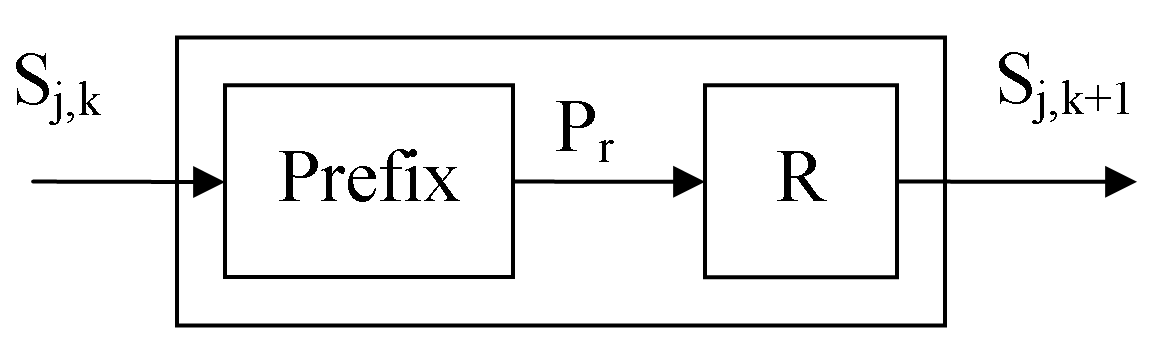
\includegraphics[width=3in]{./figures/mapping-function-stream.PNG}
	\caption{Mapping function for stream ciphers}	
	\label{fig:mapping-function-stream}
\end{figure}

The state $S_{j,1}$ is then used to compute $S_{j,2}$ and the process is repeated for $t$ such computations, at the end of which the last state $S_{j,t}$ is known. The mapping function $f_i$ is shown in the figure \ref{fig:mapping-function-stream} for such a transformation. The last state is referred to as end state and denoted by $EP_j$. In all, $m$ chains are created in this way as part of one table. The same is repeated for other tables but with different reduction functions, in order to avoid collision between different tables. 

The precomputation time $P$ for this phase is $mt^2/D$, as discussed before. Since the number of tables has reduced, the order of memory required to store the starting and end points of each chain also reduces. With $t/D$ tables and $m$ chains in each table, we have $M$ = $m \cdot (t/D)$.\\

\noindent \textit{\textbf{Attack phase.}} The attack phase for stream ciphers is similar to that for block ciphers. Every subsequence of the keystream is searched in all the tables. The possibility of the current state occurring in one of the columns of a table is checked for each of the $t/D$ tables. In the worst case for searching one prefix, $t$ computations are required per table which amounts to $t \cdot (t/D)$ computations for the entire table structure. For searching through $D$ prefixes, the time required is $t^2$. Hence the worst case attack time is of the order of $t^2$ and we have $T$ = $t^2$.\\

\noindent \textit{\textbf{Tradeoff equation.}} The tradeoff equation can be easily derived by eliminating the parameters $m$ and $t$ from the following three important equations,
\begin{align*}
M &= mt/D\\
T &= t^2\\
mt^2 &= N
\end{align*}
The tradeoff equation comes out to be,
\begin{align}
\label{eq:tmdto-hellman-stream} TM^2D^2 = N^2
\end{align}
  \\
\noindent \textit{\textbf{A general tradeoff equation.}} The tradeoff equation derived above is proposed in \cite{biryukov2000ctm} by Biryukov and Shamir. In the derivation of this equation, we have replaced the number of tables $r$ (the value of which is $t$ for block ciphers) with $r$ = $t/D$. We know that the parameters $r$ and $t$ determine the size of the tables and thus correspond to the precomputation phase, and $D$ on the other hand corresponds to the attack phase. Since the number of tables is such that $r \geq 1$, we have the condition that $D \leq t$. This creates a dependency of the attack phase parameter on the precomputation phase parameter. This dependency is particularly not helpful if we want to change $D$ frequently with a fixed precomputation table. The precomputation phase in such a case would have to be carried out again with the new $D$ in consideration, before the attack could be mounted. 

Here, we describe a different and simpler form of the tradeoff equation, which uses the parameter $r$ in the precomputation phase without replacing it with $t/D$. Thus, if there are $r$ tables, with each table having $mt$ states, then the total number of states in the Hellman table structure is $mtr$. During the attack phase, $D$ states are traversed through, thus the product $mtr \cdot D$ must be $N$. Hence we have, 
\begin{align}
\label{eq:tmdto-hellman-general} mtr \cdot D = N
\end{align}
We call the equation \ref{eq:tmdto-hellman-general} as the general tradeoff equation for TMDTO attacks on stream ciphers using Hellman tables. Using this equation, the parameters $m$, $t$, $r$ and $D$ can be set independent of each other thus offering a greater flexibility while running the attack. Following these parameters, $T$ and $M$ can be calculated as follows.
\begin{align}
\label{eq:tmdto-hellman-general-memory} M &= mr\\
\label {eq:tmdto-hellman-general-time} T &= trD
\end{align}
In the next section results of the performance of Hellman tables on HiTag2 cipher are provided. The parameters used for these results are taken from the general tradeoff equation. Furthermore, the Biryukov and Shamir tradeoff equation is used for comparison with rainbow table in section \ref{sec:compare-hellman-rainbow}.

\section{Implementation and results}
\label{sec:hellman-table-impl}

The implementation of the Hellman tables for stream ciphers differs from the implementation of previously discussed TMTO attacks in certain ways. For every table a separate hashtable is constructed. This is because every table has its own reduction function. Each table is identified by a table number $i$ such that $1 \geq i \geq r$. The reduction function used for the table $i$ is shown in equation \ref{eq:reduction-function}, where $k$ represents a column in the chain $j$.

\begin{align}
\label{eq:reduction-function} S_{j,k+1} = f_i(S_{j,k}) = R_i(Prefix(S_{j,k})) = Prefix(S_{j,k}) \oplus i
\end{align}  

As can be seen, $R_i$ is basically an \textit{xor} between the prefix and the table number. This ofcourse is a very simple reduction function and more complicated functions can be constructed. Though in the literal sense, $R_i$ is not behaving as a reduction function since the input (the prefix) and output (next state) of the function have the same length of 48 bits. This function is rather a permutation function and maps one element in the prefix space to another element in the same space. If prefixes of length 56 bits are used, then these 56 bits must be mapped to 48 bits of state. In such a case, the terminology for the reduction function would be appropriate. But, we continue using the same name in the case of 48 bit prefixes in order to avoid creating new terms for special cases. 

In the implementation, we execute a separate program to carry out the precomputation phase of the attack. This program computes the starting and end points for each table and stores them in an ASCII file on the local disk. The reason for doing this is that the precomputation takes hours to complete, for example for $P = 2^{33}$, the time taken is 13 hours. Hence, storing the tables in a file is a better idea instead of generating the precomputation tables each time the attack is executed. The size of precomputation files for all the used parameters is given in appendix \ref{app:size-precomp-files}.

The following steps are performed in sequence as part of the complete attack. 

\begin{enumerate}
\item The Hellman tables are created for given parameters $m,t,r$ and $D$, and stored in a file on the hard disk. This program is not part of the attack module.
\item The first step in the attack module is to prepare the hashtables by reading the file. The parameters from the file are matched with the parameters expected in the attack. If they are compatible then file reading process is continued. Otherwise the program terminates. The size of each hashtable prepared is $m$. The total precomputation memory is as given by equation \ref{eq:tmdto-hellman-general-memory}. The time for precomputation $P$ is given by $mtr$.
\item Keystream is generated for the attack. The length of the keystream depends on value of $D$ chosen.
\item The attack is started. Each subsequence from the keystream is searched in the hashtable. The time for the attack is as given by equation \ref{eq:tmdto-hellman-general-time}. 
\end{enumerate}

Seven different combinations of the four parameters are chosen and the results of the attack are shown in table \ref{tab:hellman-attack-results} corresponding to the key $K_2$. Due to the extensive time taken for precomputation, we used an additional machine (Dell) for precomputation of some parameter combinations in order to create tables in parallel to the \textit{gray} server. Moreover we tried to use a same machine in the attack phase for all parameter combinations (\textit{gray} server), but due to some reason we had to switch to the \textit{glint} server for running some attacks, which was faster than the \textit{gray} server.
\begin{table}[ht!]
\begin{center}
\caption{Results of TMDTO Hellman attack for $K_2$}
\smallskip
\smallskip
\begin{threeparttable}
\begin{tabular}{|p{3.5cm}||c|c|c|c|c|c|c|}
\hline
m																				&	$2^{16}$ 	&	$2^{14}$ 	&	$2^{16}$ 	&	$2^{14}$ &	$2^{14}$ 	&	$2^{14}$ 	&	$2^{14}$	\\ 
t	  																		&	$2^{16}$ 	&	$2^{17}$ 	&	$2^{16}$ 	&	$2^{12}$ &	$2^{17}$ 	&	$2^{10}$ 	&	$2^{17}$	\\ 
r	  																		&	$2^{1}$ 	&	$2^{1}$ 	&	$2^{2}$ 	&	$2^{6}$	 &	$2^{2}$ 	&	$2^{8}$ 	&	$2^{2}$		\\ 
D	  																		&	$2^{15}$ 	&	$2^{16}$ 	&	$2^{14}$ 	&	$2^{16}$ &	$2^{15}$ 	&	$2^{16}$ 	&	$2^{16}$	\\ \hline \hline
M																				&	$2^{17}$ 	&	$2^{15}$ 	&	$2^{18}$ 	&	$2^{20}$ &	$2^{16}$ 	&	$2^{22}$ 	&	$2^{16}$	\\ 
P	  																		&	$2^{33}$ 	&	$2^{32}$ 	&	$2^{34}$ 	&	$2^{32}$ &	$2^{33}$ 	&	$2^{32}$ 	&	$2^{33}$	\\ 
T	  																		&	$2^{32}$ 	&	$2^{34}$ 	&	$2^{32}$ 	&	$2^{34}$ &	$2^{34}$ 	&	$2^{34}$ 	&	$2^{35}$	\\ \hline \hline
Precomputation time for file (hours)		&	13 	 			&	6.5 			&	36.7 \tnote{a}	&	7.3&	13 	 			&	9.2 \tnote{a} &	13		\\ \hline
Time for attack	(hours)									&	6.7 			&	25.2			&	1.8	 \tnote{b}	&	25 &	6.43 \tnote{b}&	7.3 \tnote{b}	&	12.8 \tnote{b}	\\ \hline
Number of times correct key is found 		&	2 				&	1					&	2 				&	0 			 &	0 	 			&	1   			&	2				\\ \hline
Time of first correct key (hours)				&	1.2 			&	24.0			&	0.6	 		 	&	-		 		 &	- 	 			&	4.1 			&	9.2			\\ \hline
Number of times false key is found			&	0 				&	1 				&	1					&	5				 &	0 	 			&	2 				&	2				\\ \hline
Number of false alarms									&	33K 			&	66.6K			&	33.3K			&	2K			 &	67K 			&	0.5K			&	134K		\\ \hline
\end{tabular}
\smallskip
\begin{tablenotes}
	\item[a] The precomputation for these parameters was done on a Dell personal computer with a 2GHz Intel Centrino processor and running Ubuntu OS through LiveCD.
	\item[b] The attack is run on the \textit{glint} servers which are less busy as compared to the \textit{gray} servers used for the other attacks. Hence, the time taken for these attacks is less as compared to other attacks.
\end{tablenotes}
\end{threeparttable}
\end{center}
\label{tab:hellman-attack-results}
\end{table}

The following comments can be made based on these results.
\begin{enumerate}
\item The time for the attack and the time for precomputation are as expected for the same machines. On the Dell machine, precomputation time of $2^{32}$ takes around 9.2 hours while precomputation of $2^{34}$ takes around 4 times more than that i.e.~36.7 hours. Similarly, the attack time on the two machines \textit{glint} and \textit{gray} are seen to be proportional, which is expected.

\item It is clearly seen that as the number of tables is increased by keeping $P$ constant, the number of false alarms observed is drastically reduced. For $2^{2}$ tables, the number of false alarms is around 33000, while they reduce to around 2000 for $2^{6}$ tables. Hence, false alarms reduce by the factor by which the number of tables is increased. Further, for $r$ = $2^{8}$ only 531 false alarms are observed. Hence, it is concluded that the number of tables should be kept high.

From another point of view, it can also be concluded that the table stopping rule used to limit a table size with the aim of less collisions, is not providing us the correct upper bound on $m$ and $t$. For the results in column 4, the value of $mt^2$ is $2^{38}$. This value is much less than the maximum value suggested according to the table stopping rule, and as we can see it gives far less false alarms. This shows that the rule is not very efficient, and we are better off only when using values for $m$ and $t$ which are much lesser than those suggested by the rule. 

\item Having more number of tables does not guarantee the key to be found. We see the case in column 4 for which the correct key is not found inspite of choosing the parameters according to the general tradeoff equation. The correct key is not found for parameters in column 5 as well, but when we double $D$ for the same precomputation parameters (as shown in column 7) the correct key is found once. 

\item The parameter combination $2^{14}$-$2^{10}$-$2^{8}$-$2^{16}$ provides the best result, in terms of the number of false alarms and the time for the attack\footnote{Attack time is less as a faster machine is used; but even with the slower machine (\textit{gray}) the time would be around 25 hours, which is okay}. Ofcourse, the downside of this parameter combination is the memory requirement which is $2^{22}$ and is the most among all the parameter combinations. $2^{22}$ is not a very high requirement for memory though. If we intend to reduce $M$ and still keep $r$ the same, in order to have same $P$ we would need to increase $t$. And increasing $t$ implies increasing the attack time, which might not be a good tradeoff. 

\item There are false keys also found on several occasions during the attack. This must not be mistaken with the false alarms. False keys arise because of a prefix having more than one generating state or preimage. As a result, the prefix correctly exists in one of the Hellman tables, but with the wrong state as its preimage. This state is found by the attack, resulting in a wrong key being computed. We call such cases as false keys, and stress that they are different from false alarms. The only way of avoiding false keys is by increasing the length of prefix to 56 bits. As we have seen for TMTO keystream and tags attacks, 56 bits of prefix is sufficient in order to suppress false keys. 

\item On a positive note, the advantage of selecting the general tradeoff equation over the tradeoff by Biryukov and Shamir in order to vary the parameters is clearly seen. In the latter case we would have to fix $r$ according to $D$ and thus would not be able to observe the results by varying $r$ independently. The former tradeoff gives us this flexibility and we can make some important observations using it. 
\end{enumerate}